\documentclass[10pt, a4paper]{article}
\usepackage[margin=1.5cm]{geometry}
\usepackage{graphicx}
\usepackage{booktabs}
\usepackage{subcaption}
\usepackage{float}
\usepackage{amsmath}
\usepackage{mathpazo}
\usepackage[utf8]{inputenc}
\usepackage[T2A]{fontenc}
\usepackage[english,russian]{babel}
\usepackage{xcolor}

\title{BISTRO Polarimetric Report: Statistical Data Passport}
\author{Automated Analysis Pipeline}
\date{\today}

\begin{document}
\maketitle

\section*{Methodology and Data Integrity}
This report provides a quantitative assessment of molecular cloud structures based on BISTRO survey data. A key feature of the current pipeline is the prioritized use of hardware-derived metadata for error propagation.

\paragraph{Noise Analysis Strategy:}
The pipeline implements a "Graceful Downgrade" logic. If the FITS headers and HDU structure (derived from the STARLINK \texttt{pol2map} reduction) contain \texttt{VARIANCE} and \texttt{QUALITY} extensions, these are utilized as the primary source of per-pixel uncertainty. This accounts for the non-uniform noise distribution inherent in the JCMT \textit{Daisy Scan} pattern. In the absence of such layers, the system reverts to a heuristic estimation of the RMS within a geometric safety zone, utilizing iterative sigma-clipping to isolate the background from the emission.

\paragraph{Debiasing and Physics:}
To counteract the systematic overestimation of polarized intensity in low SNR regimes (Ricean bias), we apply the \textbf{Wardle \& Kronberg (1974)} debiasing technique: $PI_{db} = \sqrt{PI^2 - \sigma_{PI}^2}$. Pixels failing the $SNR_{PI} > 2$ criterion are excluded from the structure function analysis to prevent noise-driven artifacts in the magnetic field morphology.
\newpage\section*{Target: Auriga}
\begin{table}[H]
    \centering
    \caption*{Physical Parameters and Noise Methodology}
    \begin{tabular}{lp{10cm}}
        \toprule \textbf{Parameter} & \textbf{Value} \\ \midrule
        Method I & \textbf{Hardware QUALITY Mask} \\
        Method QU & \textbf{Hardware Variance} \\
        Effective Pixels & 1502 \\
        R\_range\_pc & 0.0087 -- 1.5708 \\
        Distance (pc) & 450.00000 \\
        R\_range\_px & [1, 180] \\
        Vector Decimation Step & 3 px \\
        \bottomrule
    \end{tabular}
\end{table}

\begin{figure}[H]
    \centering
    \begin{subfigure}{0.48\textwidth} 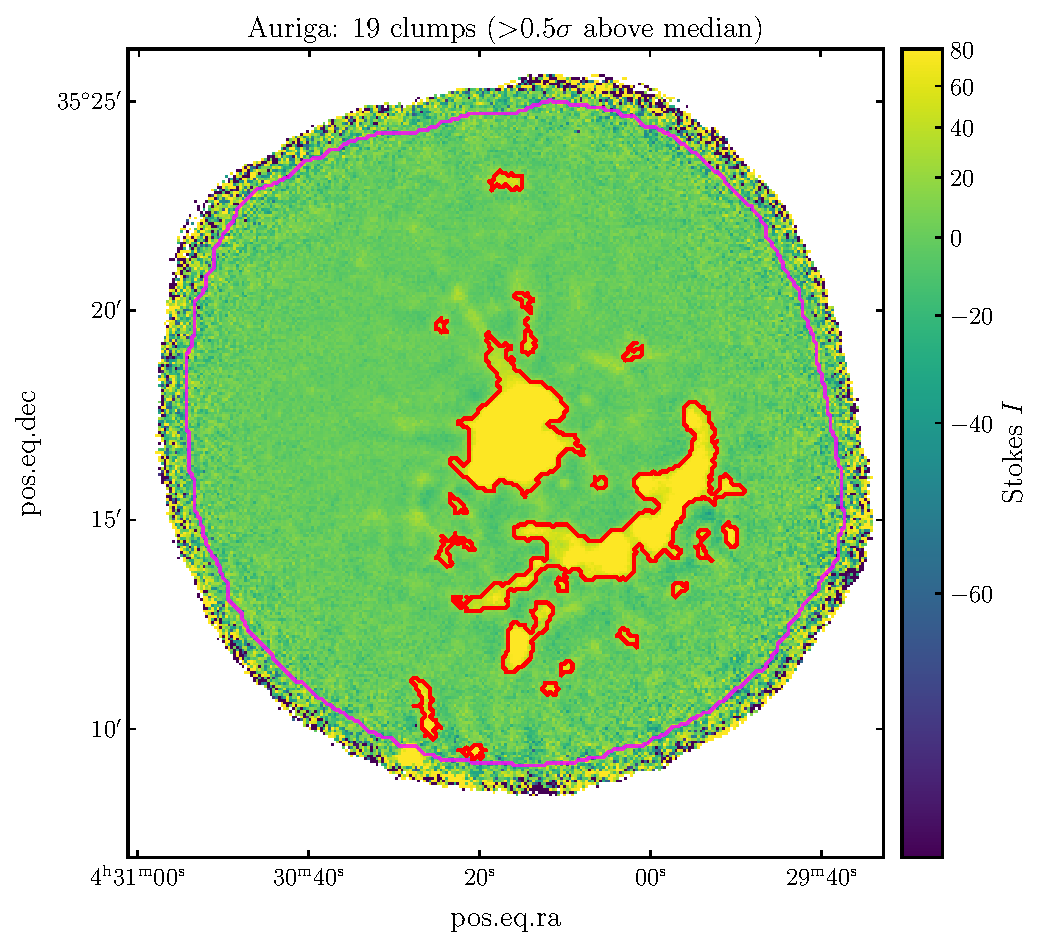
\includegraphics[width=\linewidth]{../plots/Auriga/Auriga_stat_segmentation.pdf} 
    \caption{Segmentation \& Clump Masking} \end{subfigure} \hfill
    \begin{subfigure}{0.48\textwidth} 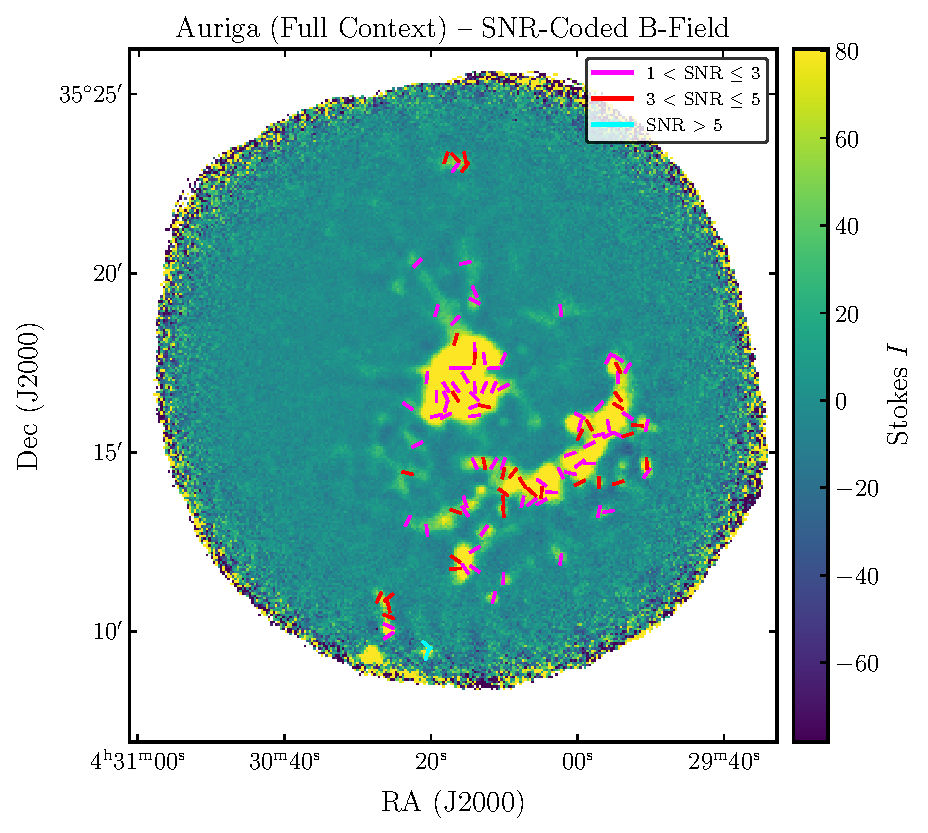
\includegraphics[width=\linewidth]{../plots/Auriga/Auriga_snr_colored_full.pdf} 
    \caption{SNR-Coded B-Field Vectors} \end{subfigure}
    \vspace{0.5cm}
    \begin{subfigure}{0.7\textwidth} 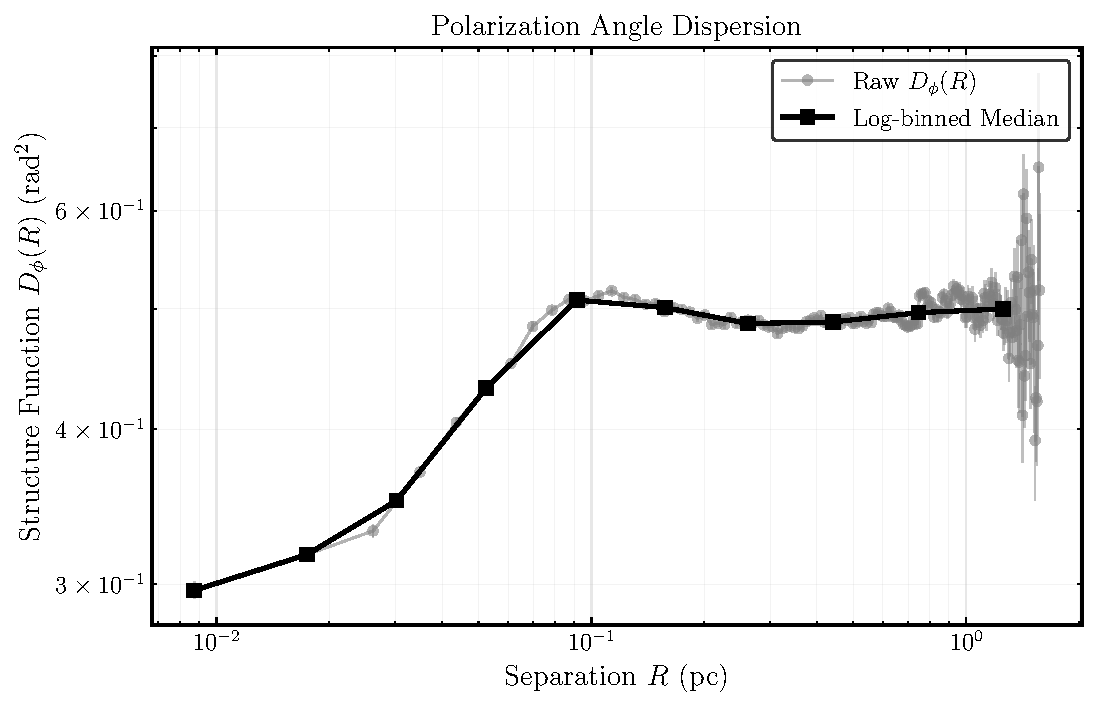
\includegraphics[width=\linewidth]{../plots/Auriga/Auriga_sf.pdf} 
    \caption{Structure Function $D_\phi(R)$} \end{subfigure}
\end{figure}
\newpage
\section*{Target: L1495}
\begin{table}[H]
    \centering
    \caption*{Physical Parameters and Noise Methodology}
    \begin{tabular}{lp{10cm}}
        \toprule \textbf{Parameter} & \textbf{Value} \\ \midrule
        Method I & \textbf{Hardware QUALITY Mask} \\
        Method QU & \textbf{Hardware Variance} \\
        Effective Pixels & 78 \\
        R\_range\_pc & 0.0054 -- 0.4941 \\
        Distance (pc) & 140.00000 \\
        R\_range\_px & [1, 91] \\
        Vector Decimation Step & 3 px \\
        \bottomrule
    \end{tabular}
\end{table}

\begin{figure}[H]
    \centering
    \begin{subfigure}{0.48\textwidth} 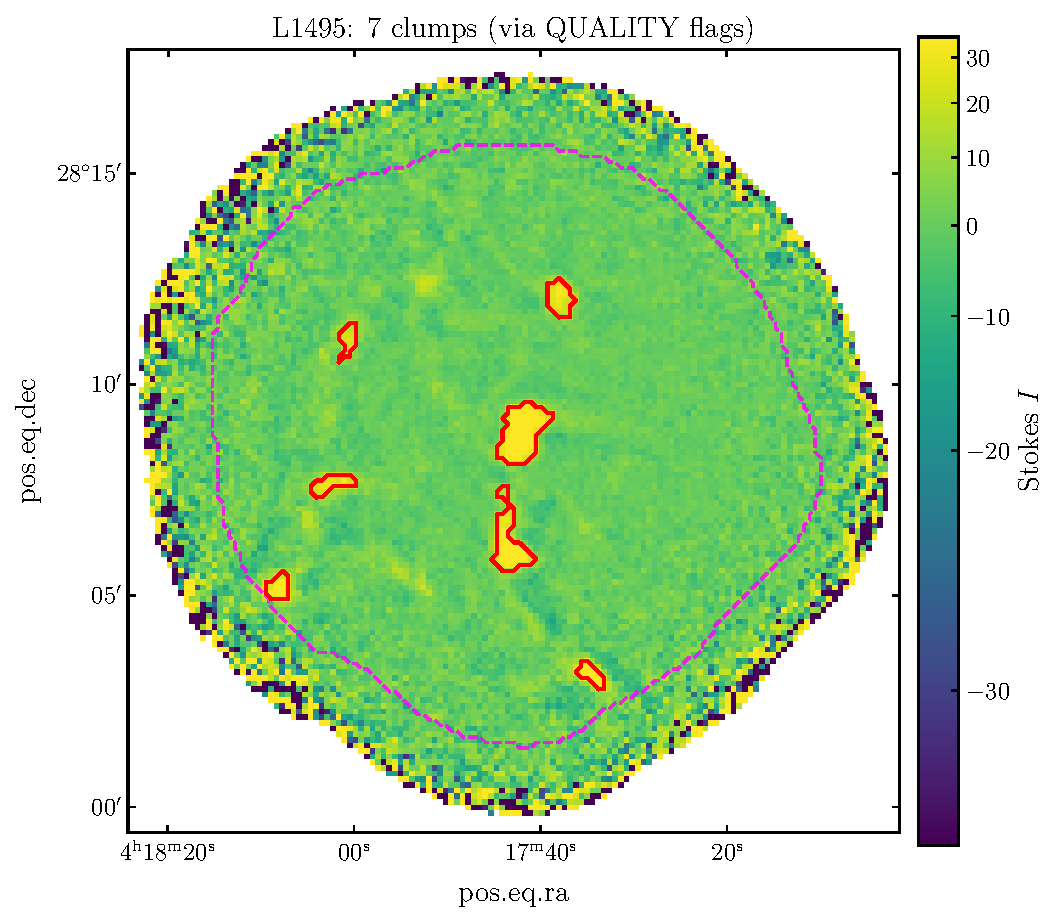
\includegraphics[width=\linewidth]{../plots/L1495/L1495_stat_segmentation.pdf} 
    \caption{Segmentation \& Clump Masking} \end{subfigure} \hfill
    \begin{subfigure}{0.48\textwidth} 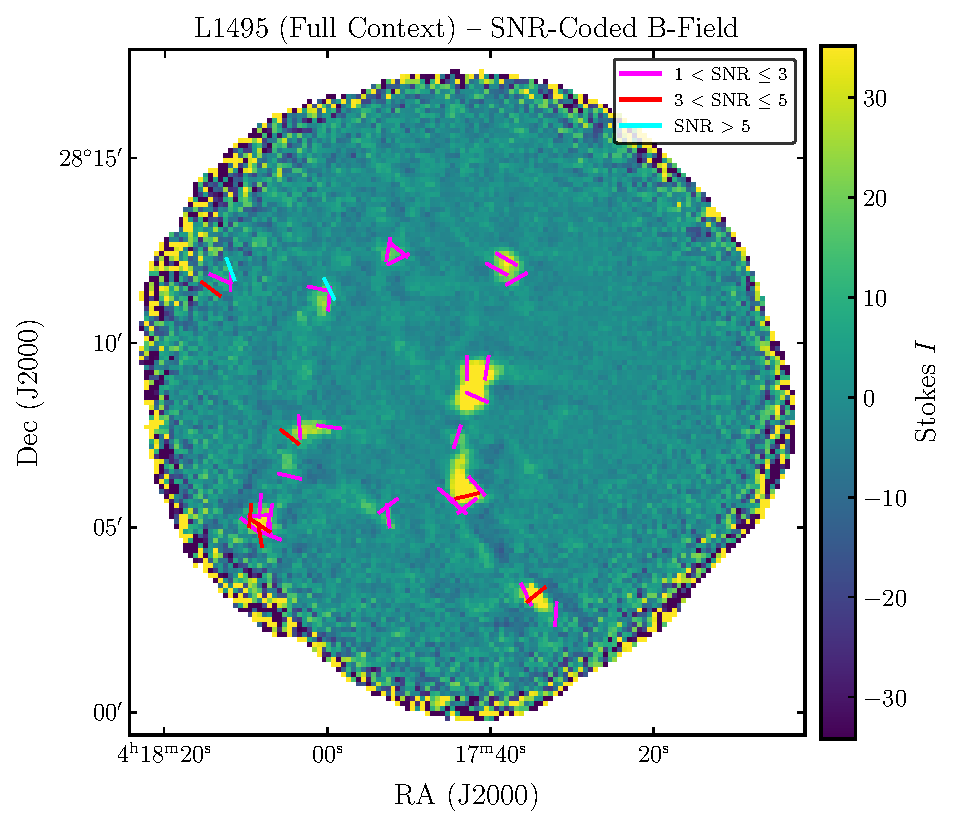
\includegraphics[width=\linewidth]{../plots/L1495/L1495_snr_colored_full.pdf} 
    \caption{SNR-Coded B-Field Vectors} \end{subfigure}
    \vspace{0.5cm}
    \begin{subfigure}{0.7\textwidth} 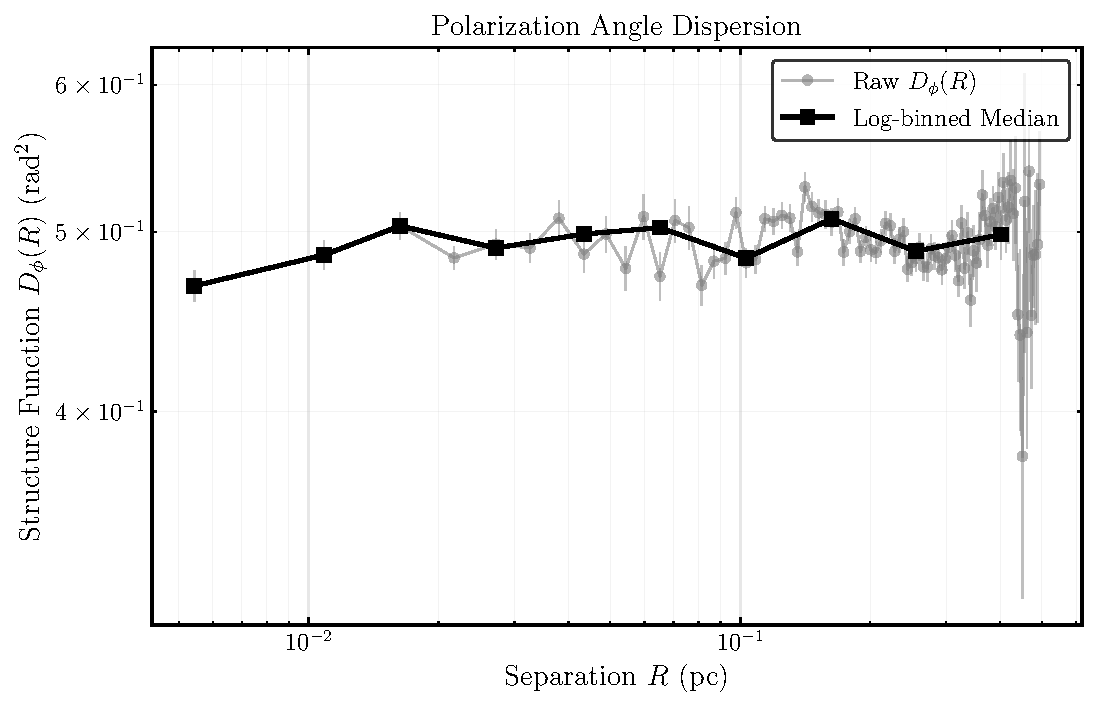
\includegraphics[width=\linewidth]{../plots/L1495/L1495_sf.pdf} 
    \caption{Structure Function $D_\phi(R)$} \end{subfigure}
\end{figure}
\newpage
\section*{Target: L43\_Karoly\_2023}
\begin{table}[H]
    \centering
    \caption*{Physical Parameters and Noise Methodology}
    \begin{tabular}{lp{10cm}}
        \toprule \textbf{Parameter} & \textbf{Value} \\ \midrule
        Method I & \textbf{Hardware QUALITY Mask} \\
        Method QU & \textbf{Hardware Variance} \\
        Effective Pixels & 189 \\
        R\_range\_pc & 0.0048 -- 0.4266 \\
        Distance (pc) & 125.00000 \\
        R\_range\_px & [1, 88] \\
        Vector Decimation Step & 2 px \\
        \bottomrule
    \end{tabular}
\end{table}

\begin{figure}[H]
    \centering
    \begin{subfigure}{0.48\textwidth} 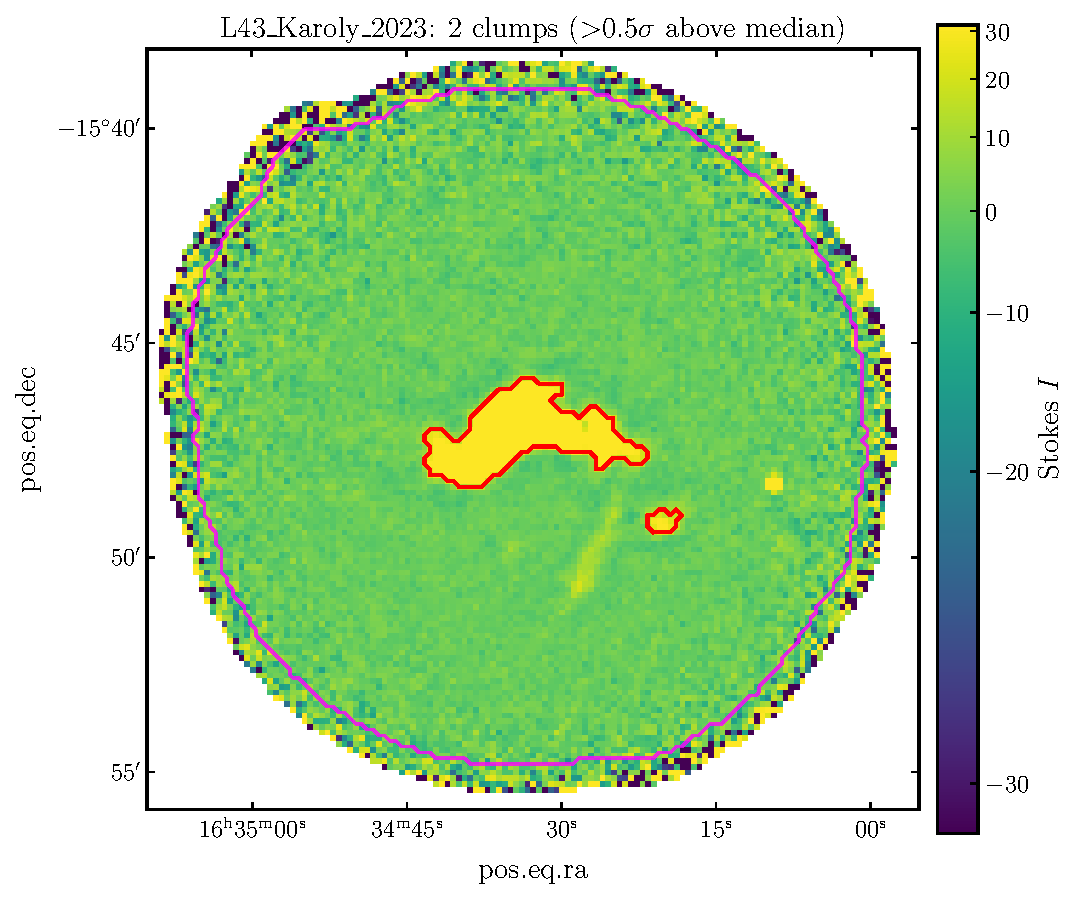
\includegraphics[width=\linewidth]{../plots/L43_Karoly_2023/L43_Karoly_2023_stat_segmentation.pdf} 
    \caption{Segmentation \& Clump Masking} \end{subfigure} \hfill
    \begin{subfigure}{0.48\textwidth} 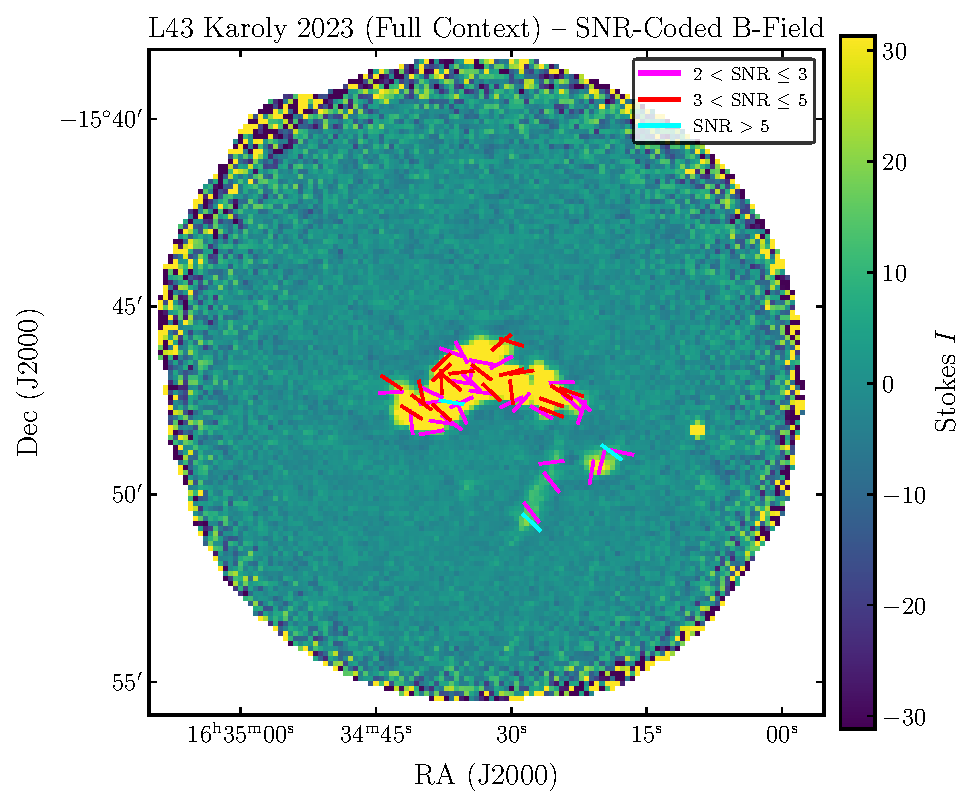
\includegraphics[width=\linewidth]{../plots/L43_Karoly_2023/L43_Karoly_2023_snr_colored_full.pdf} 
    \caption{SNR-Coded B-Field Vectors} \end{subfigure}
    \vspace{0.5cm}
    \begin{subfigure}{0.7\textwidth} 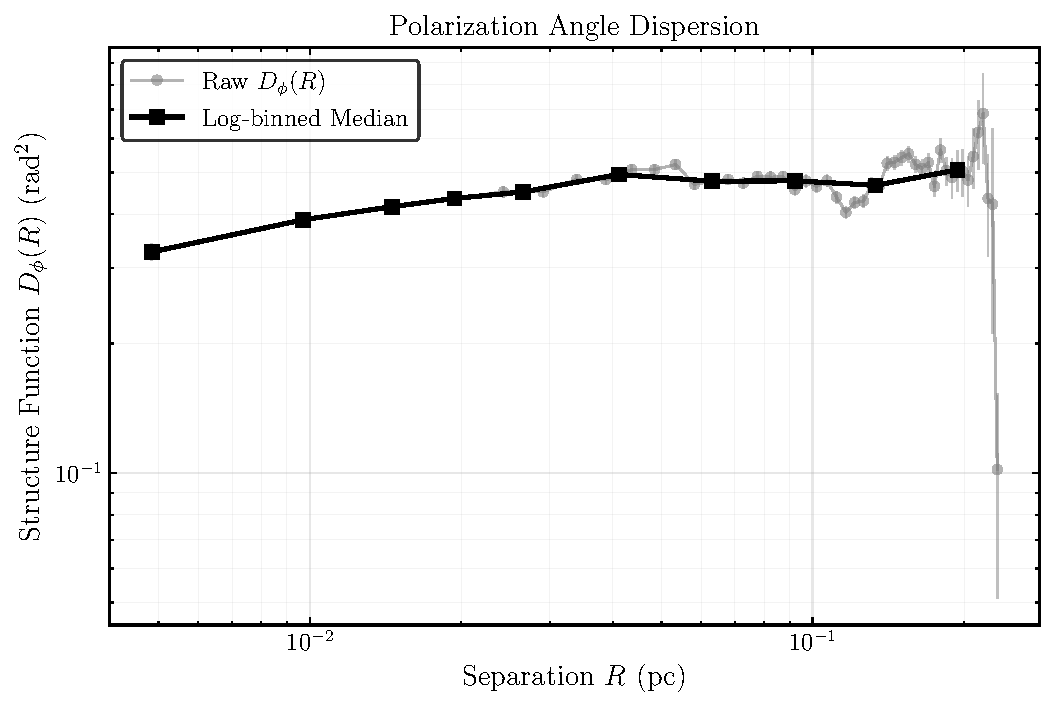
\includegraphics[width=\linewidth]{../plots/L43_Karoly_2023/L43_Karoly_2023_sf.pdf} 
    \caption{Structure Function $D_\phi(R)$} \end{subfigure}
\end{figure}
\newpage
\section*{Target: MonR2}
\begin{table}[H]
    \centering
    \caption*{Physical Parameters and Noise Methodology}
    \begin{tabular}{lp{10cm}}
        \toprule \textbf{Parameter} & \textbf{Value} \\ \midrule
        Method I & \textbf{Hardware QUALITY Mask} \\
        Method QU & \textbf{Hardware Variance} \\
        Effective Pixels & 4402 \\
        R\_range\_pc & 0.0161 -- 2.8329 \\
        Distance (pc) & 830.00000 \\
        R\_range\_px & [1, 176] \\
        Vector Decimation Step & 3 px \\
        \bottomrule
    \end{tabular}
\end{table}

\begin{figure}[H]
    \centering
    \begin{subfigure}{0.48\textwidth} 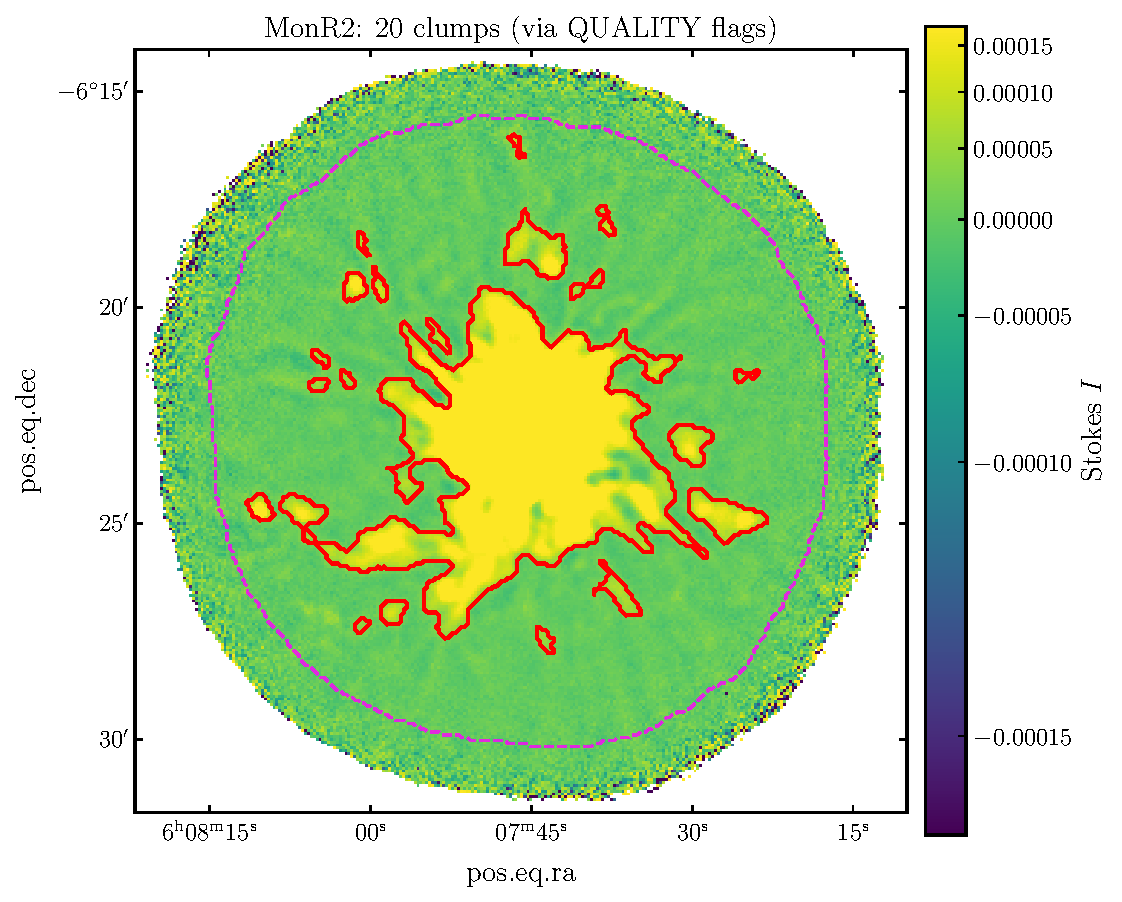
\includegraphics[width=\linewidth]{../plots/MonR2/MonR2_stat_segmentation.pdf} 
    \caption{Segmentation \& Clump Masking} \end{subfigure} \hfill
    \begin{subfigure}{0.48\textwidth} 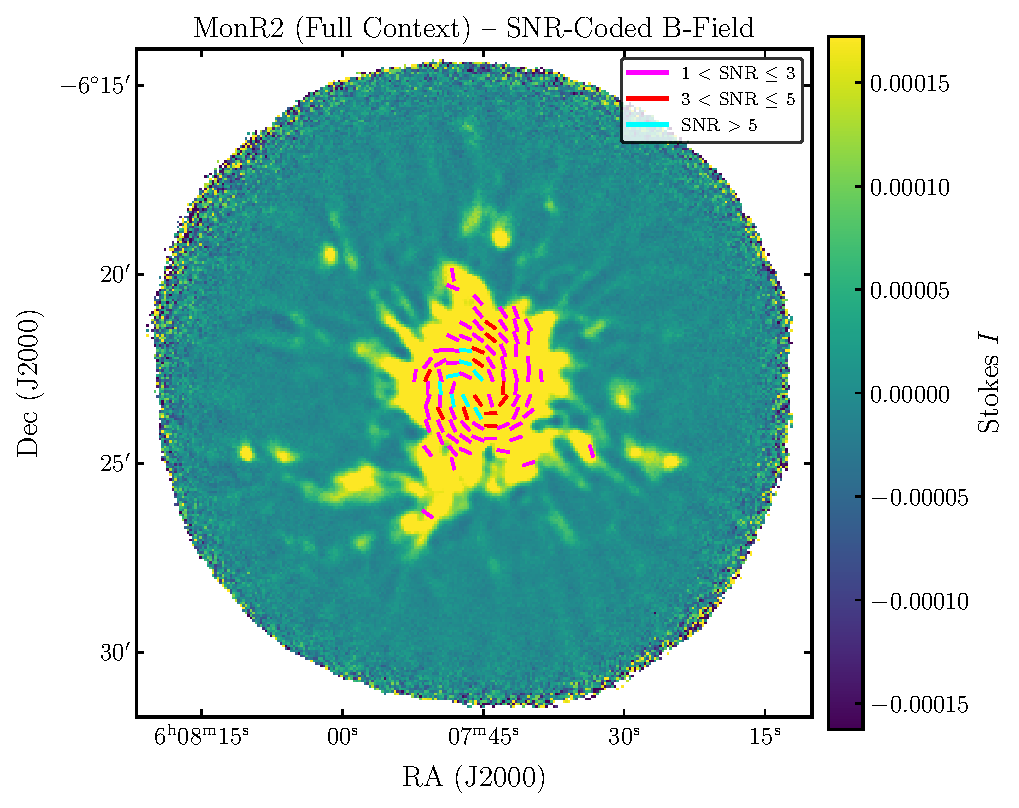
\includegraphics[width=\linewidth]{../plots/MonR2/MonR2_snr_colored_full.pdf} 
    \caption{SNR-Coded B-Field Vectors} \end{subfigure}
    \vspace{0.5cm}
    \begin{subfigure}{0.7\textwidth} 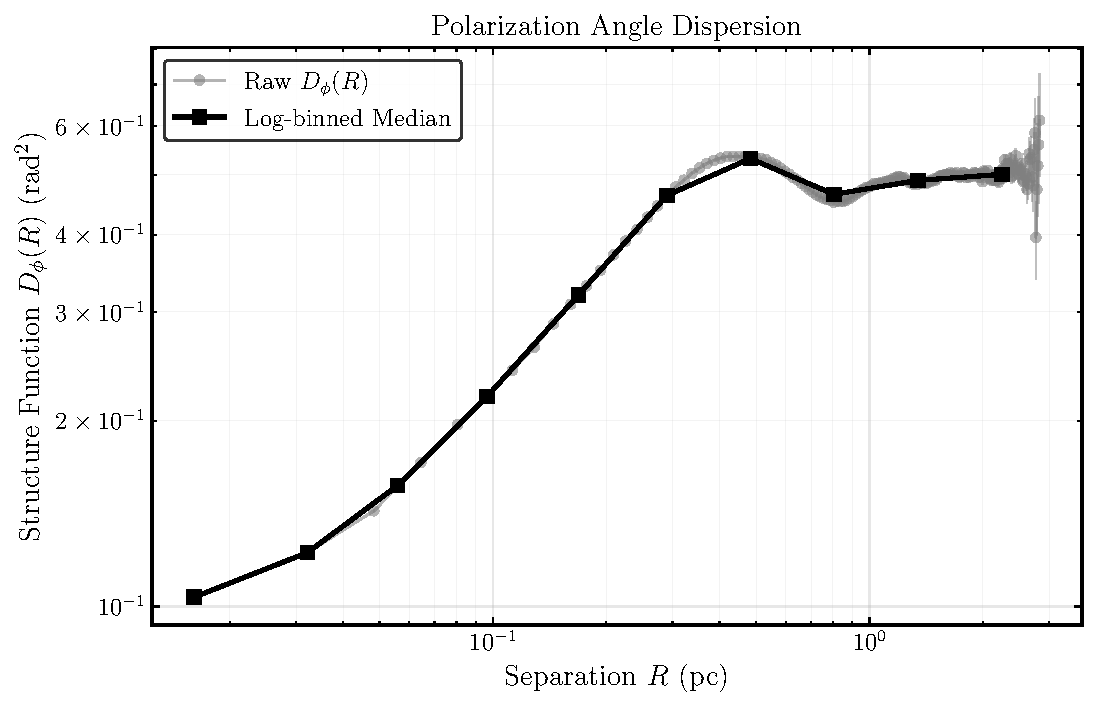
\includegraphics[width=\linewidth]{../plots/MonR2/MonR2_sf.pdf} 
    \caption{Structure Function $D_\phi(R)$} \end{subfigure}
\end{figure}
\newpage
\section*{Target: NGC1333}
\begin{table}[H]
    \centering
    \caption*{Physical Parameters and Noise Methodology}
    \begin{tabular}{lp{10cm}}
        \toprule \textbf{Parameter} & \textbf{Value} \\ \midrule
        Distance & 299.0 pc \\
        \textit{Data Status} & \color{red}\textit{Stats JSON missing (Heuristic Fallback implied)} \\
        Vector Decimation Step & 3 px \\
        \bottomrule
    \end{tabular}
\end{table}

\begin{figure}[H]
    \centering
    \begin{subfigure}{0.48\textwidth} 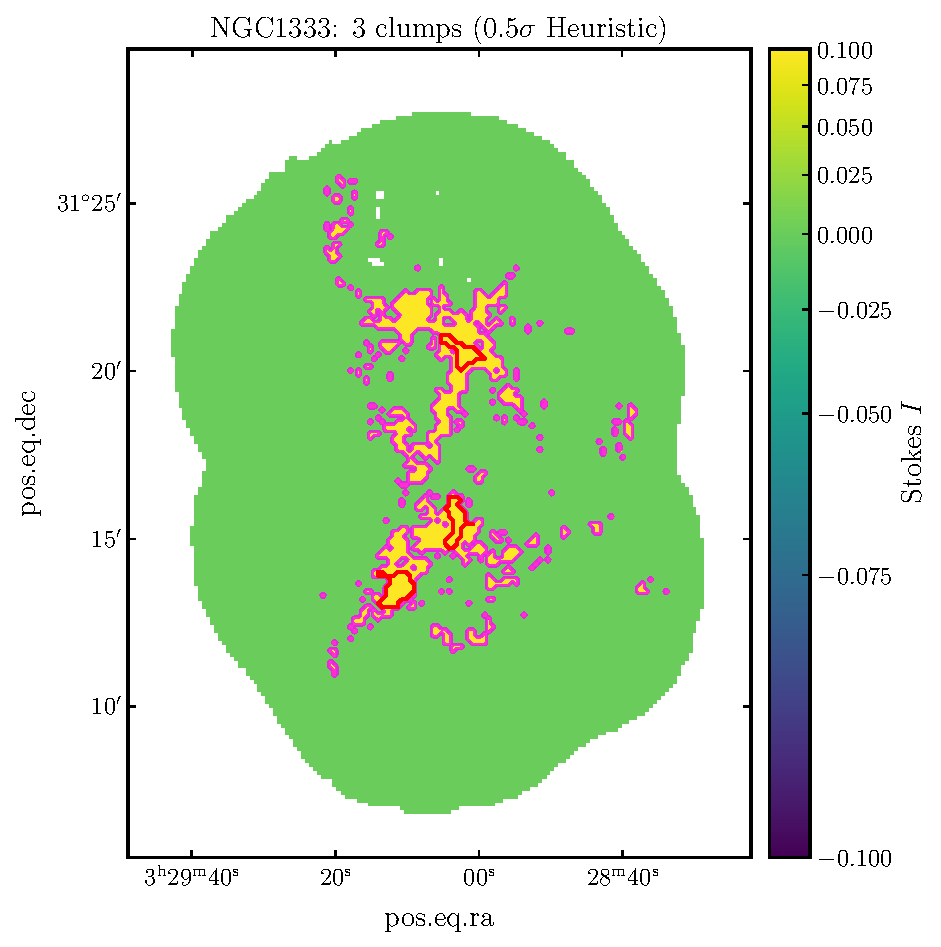
\includegraphics[width=\linewidth]{../plots/NGC1333/NGC1333_stat_segmentation.pdf} 
    \caption{Segmentation \& Clump Masking} \end{subfigure} \hfill
    \begin{subfigure}{0.48\textwidth} 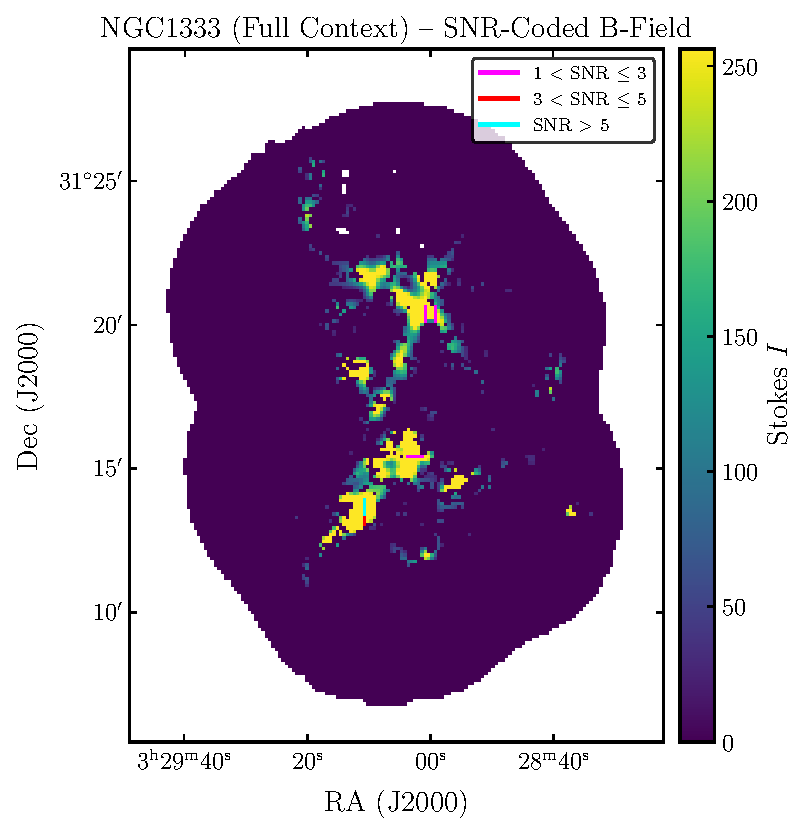
\includegraphics[width=\linewidth]{../plots/NGC1333/NGC1333_snr_colored_full.pdf} 
    \caption{SNR-Coded B-Field Vectors} \end{subfigure}
    \vspace{0.5cm}
    \begin{subfigure}{0.7\textwidth} 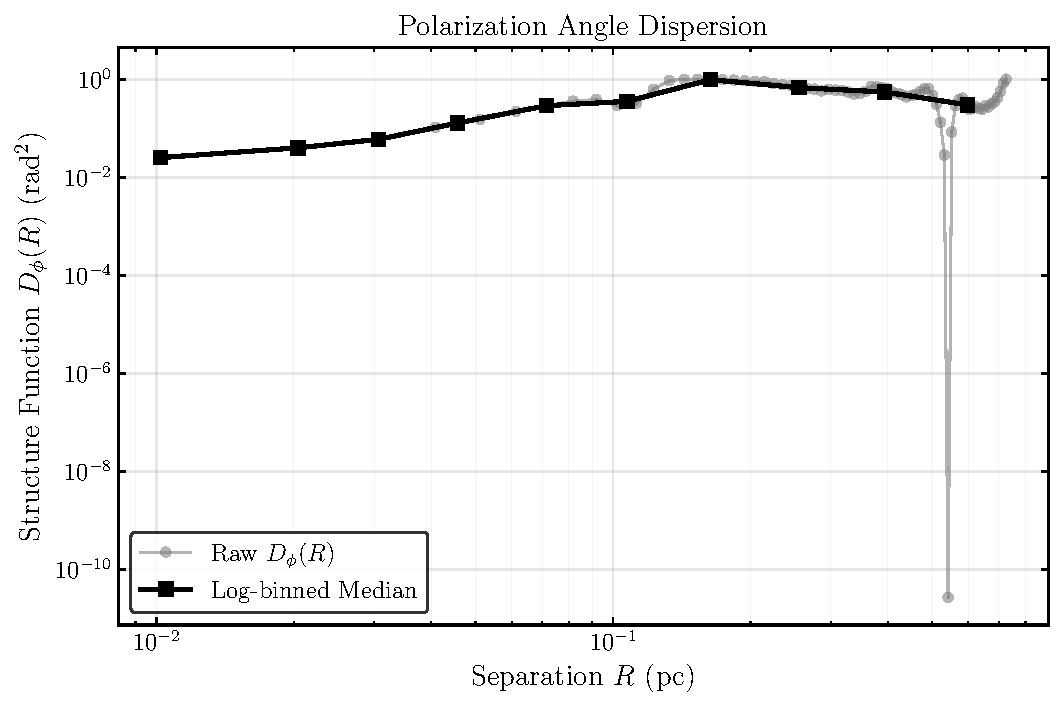
\includegraphics[width=\linewidth]{../plots/NGC1333/NGC1333_sf.pdf} 
    \caption{Structure Function $D_\phi(R)$} \end{subfigure}
\end{figure}
\newpage
\section*{Target: OMC1\_450}
\begin{table}[H]
    \centering
    \caption*{Physical Parameters and Noise Methodology}
    \begin{tabular}{lp{10cm}}
        \toprule \textbf{Parameter} & \textbf{Value} \\ \midrule
        Distance & 388.0 pc \\
        \textit{Data Status} & \color{red}\textit{Stats JSON missing (Heuristic Fallback implied)} \\
        Vector Decimation Step & 3 px \\
        \bottomrule
    \end{tabular}
\end{table}

\begin{figure}[H]
    \centering
    \begin{subfigure}{0.48\textwidth} 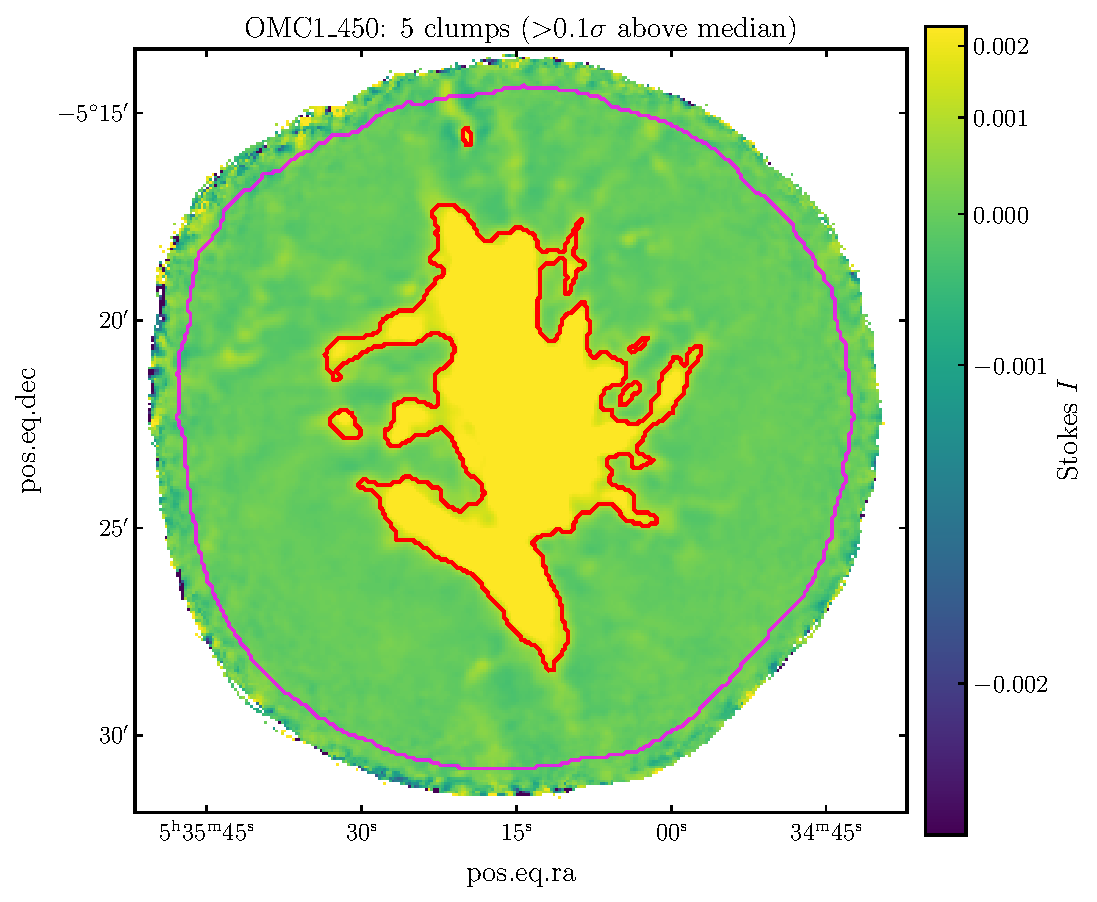
\includegraphics[width=\linewidth]{../plots/OMC1_450/OMC1_450_stat_segmentation.pdf} 
    \caption{Segmentation \& Clump Masking} \end{subfigure} \hfill
    \begin{subfigure}{0.48\textwidth} 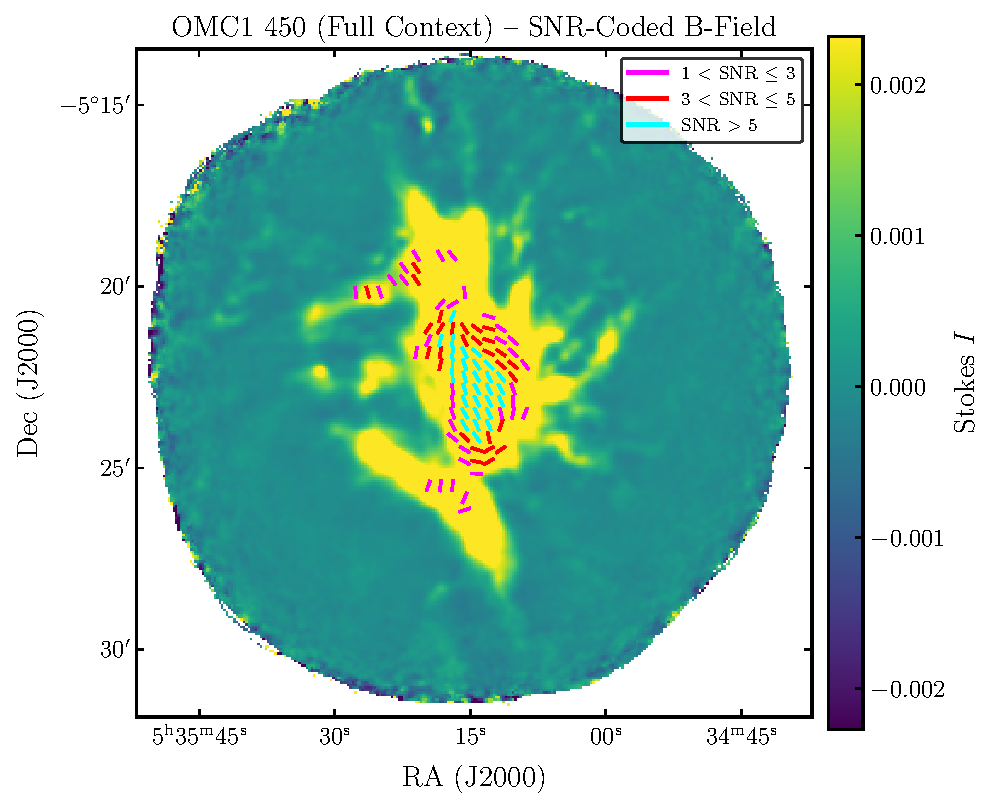
\includegraphics[width=\linewidth]{../plots/OMC1_450/OMC1_450_snr_colored_full.pdf} 
    \caption{SNR-Coded B-Field Vectors} \end{subfigure}
    \vspace{0.5cm}
    \begin{subfigure}{0.7\textwidth} 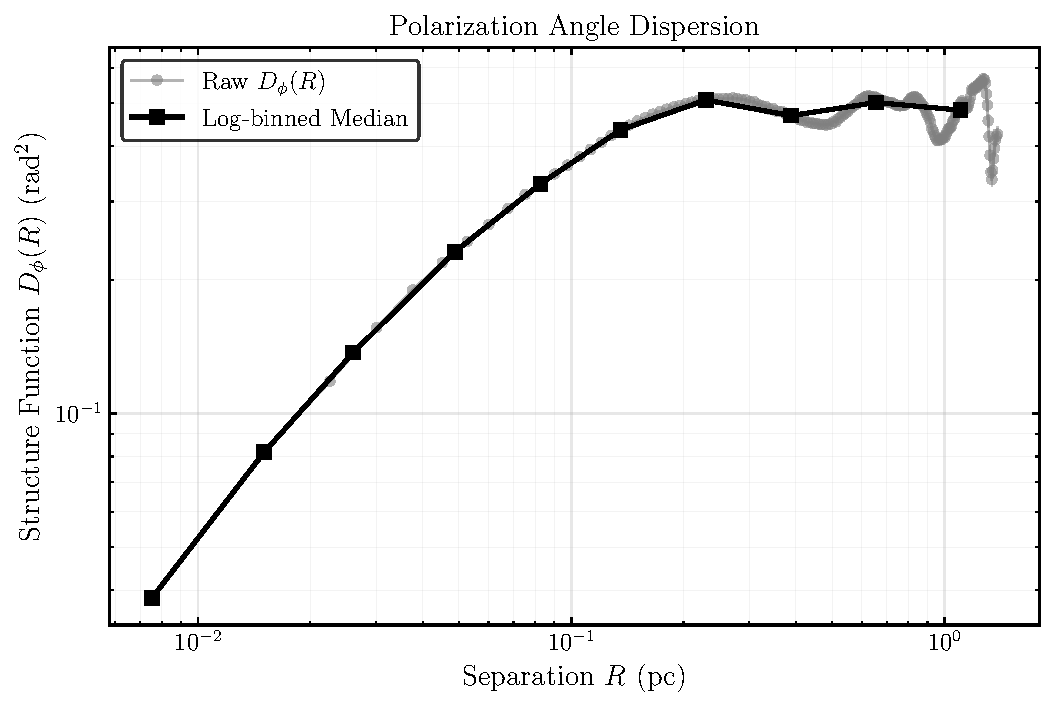
\includegraphics[width=\linewidth]{../plots/OMC1_450/OMC1_450_sf.pdf} 
    \caption{Structure Function $D_\phi(R)$} \end{subfigure}
\end{figure}
\newpage
\section*{Target: OMC1}
\begin{table}[H]
    \centering
    \caption*{Physical Parameters and Noise Methodology}
    \begin{tabular}{lp{10cm}}
        \toprule \textbf{Parameter} & \textbf{Value} \\ \midrule
        Method I & \textbf{0.1$\sigma$ Heuristic + Hardware Variance} \\
        Method QU & \textbf{Hardware Variance} \\
        Effective Pixels & 6779 \\
        R\_range\_pc & 0.0075 -- 1.3995 \\
        Distance (pc) & 388.00000 \\
        R\_range\_px & [1, 186] \\
        Vector Decimation Step & 3 px \\
        \bottomrule
    \end{tabular}
\end{table}

\begin{figure}[H]
    \centering
    \begin{subfigure}{0.48\textwidth} \includegraphics[width=\linewidth]{../plots/OMC1/OMC1_stat_segmentation.pdf} 
    \caption{Segmentation \& Clump Masking} \end{subfigure} \hfill
    \begin{subfigure}{0.48\textwidth} \includegraphics[width=\linewidth]{../plots/OMC1/OMC1_snr_colored_full.pdf} 
    \caption{SNR-Coded B-Field Vectors} \end{subfigure}
    \vspace{0.5cm}
    \begin{subfigure}{0.7\textwidth} \includegraphics[width=\linewidth]{../plots/OMC1/OMC1_sf.pdf} 
    \caption{Structure Function $D_\phi(R)$} \end{subfigure}
\end{figure}
\newpage
\section*{Target: Perseus\_B1}
\begin{table}[H]
    \centering
    \caption*{Physical Parameters and Noise Methodology}
    \begin{tabular}{lp{10cm}}
        \toprule \textbf{Parameter} & \textbf{Value} \\ \midrule
        Method I & \textbf{0.3$\sigma$ Heuristic + Hardware Variance} \\
        Method QU & \textbf{Hardware Variance} \\
        Effective Pixels & 401 \\
        R\_range\_pc & 0.0170 -- 1.0228 \\
        Distance (pc) & 293.00000 \\
        R\_range\_px & [1, 60] \\
        Vector Decimation Step & 3 px \\
        \bottomrule
    \end{tabular}
\end{table}

\begin{figure}[H]
    \centering
    \begin{subfigure}{0.48\textwidth} 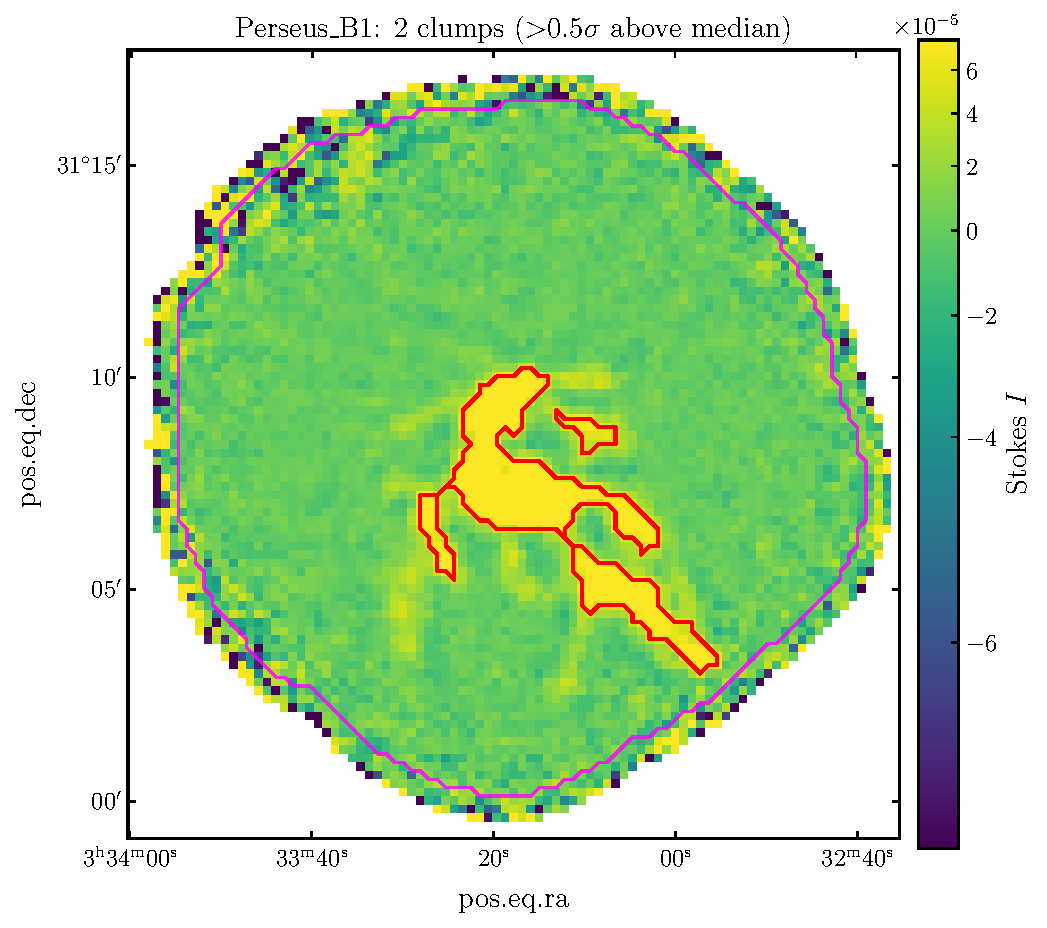
\includegraphics[width=\linewidth]{../plots/Perseus_B1/Perseus_B1_stat_segmentation.pdf} 
    \caption{Segmentation \& Clump Masking} \end{subfigure} \hfill
    \begin{subfigure}{0.48\textwidth} 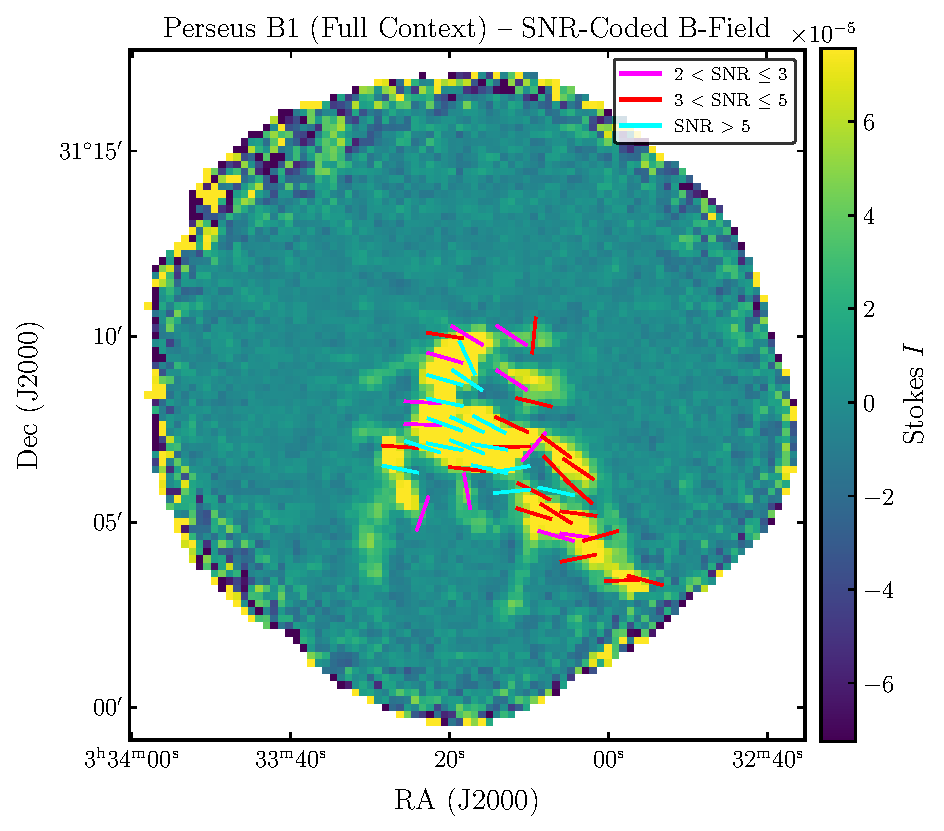
\includegraphics[width=\linewidth]{../plots/Perseus_B1/Perseus_B1_snr_colored_full.pdf} 
    \caption{SNR-Coded B-Field Vectors} \end{subfigure}
    \vspace{0.5cm}
    \begin{subfigure}{0.7\textwidth} 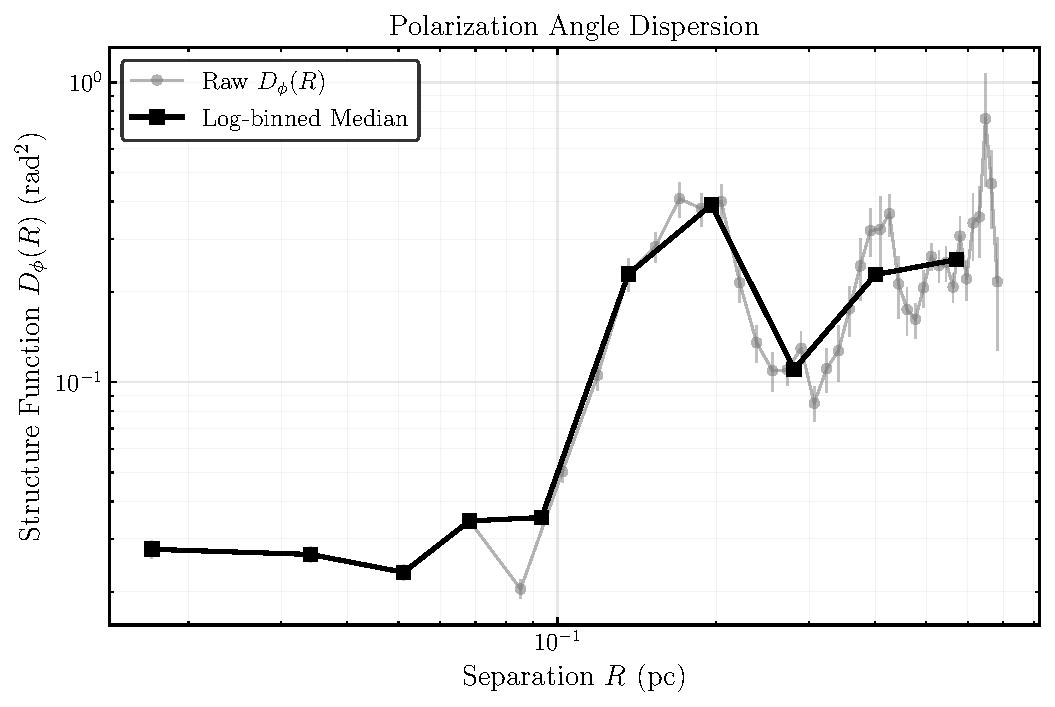
\includegraphics[width=\linewidth]{../plots/Perseus_B1/Perseus_B1_sf.pdf} 
    \caption{Structure Function $D_\phi(R)$} \end{subfigure}
\end{figure}
\newpage
\section*{Target: Rosette}
\begin{table}[H]
    \centering
    \caption*{Physical Parameters and Noise Methodology}
    \begin{tabular}{lp{10cm}}
        \toprule \textbf{Parameter} & \textbf{Value} \\ \midrule
        Method I & \textbf{Hardware QUALITY Mask} \\
        Method QU & \textbf{Hardware Variance} \\
        Effective Pixels & 1452 \\
        R\_range\_pc & 0.0258 -- 4.9005 \\
        Distance (pc) & 1330.00000 \\
        R\_range\_px & [1, 190] \\
        Vector Decimation Step & 3 px \\
        \bottomrule
    \end{tabular}
\end{table}

\begin{figure}[H]
    \centering
    \begin{subfigure}{0.48\textwidth} 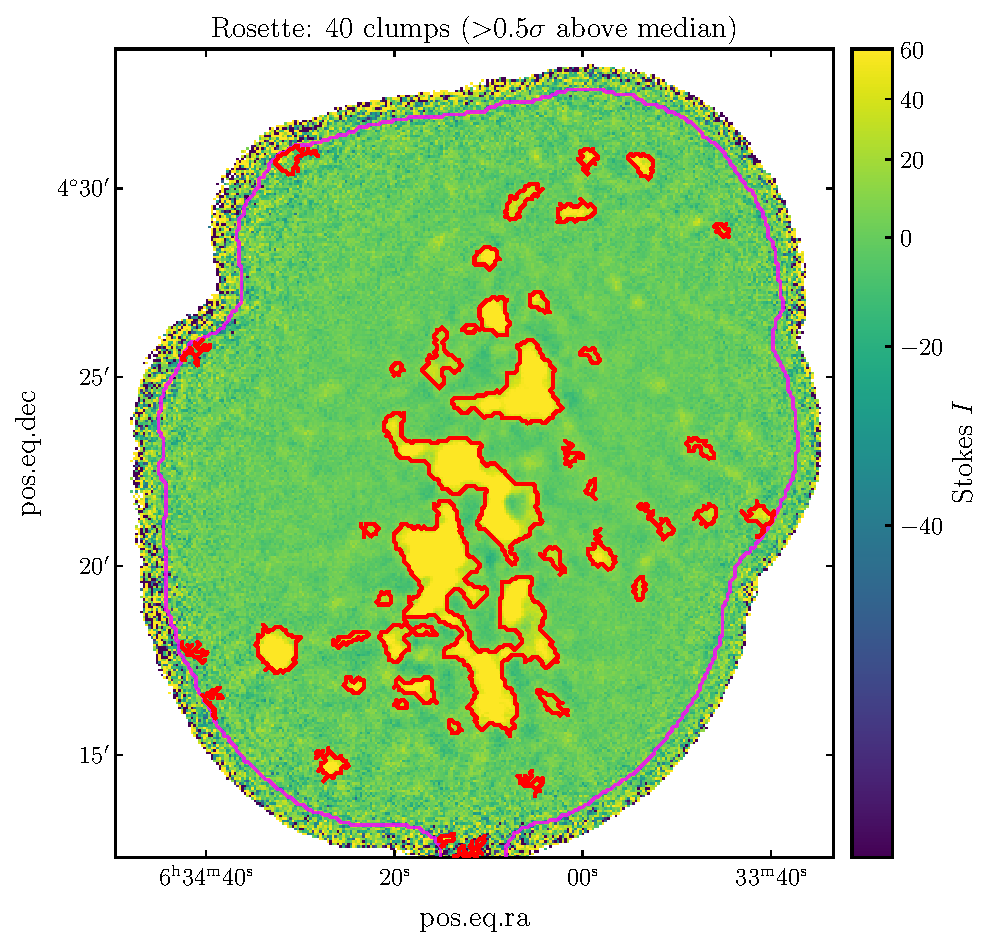
\includegraphics[width=\linewidth]{../plots/Rosette/Rosette_stat_segmentation.pdf} 
    \caption{Segmentation \& Clump Masking} \end{subfigure} \hfill
    \begin{subfigure}{0.48\textwidth} 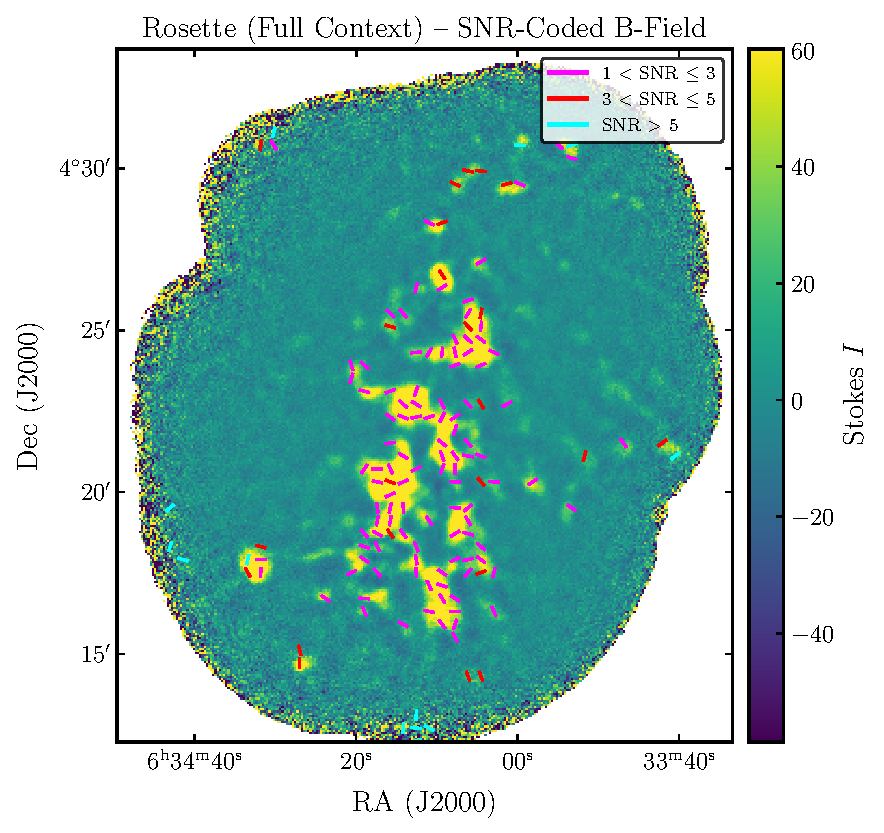
\includegraphics[width=\linewidth]{../plots/Rosette/Rosette_snr_colored_full.pdf} 
    \caption{SNR-Coded B-Field Vectors} \end{subfigure}
    \vspace{0.5cm}
    \begin{subfigure}{0.7\textwidth} 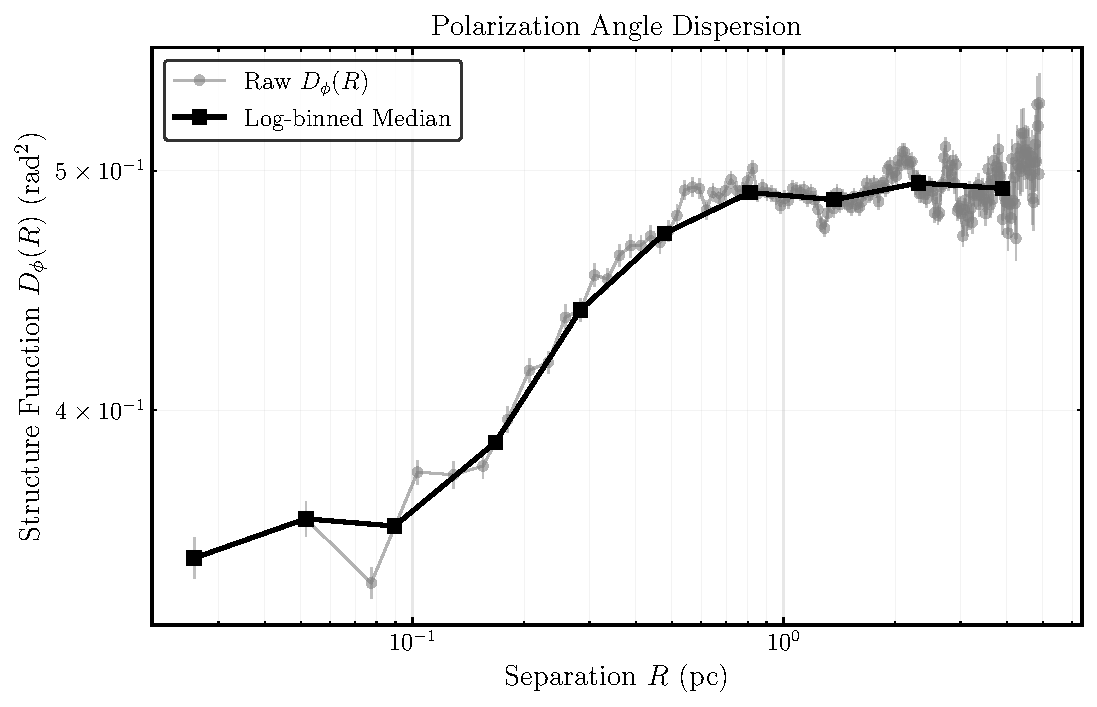
\includegraphics[width=\linewidth]{../plots/Rosette/Rosette_sf.pdf} 
    \caption{Structure Function $D_\phi(R)$} \end{subfigure}
\end{figure}
\newpage
\section*{Target: oph\_a}
\begin{table}[H]
    \centering
    \caption*{Physical Parameters and Noise Methodology}
    \begin{tabular}{lp{10cm}}
        \toprule \textbf{Parameter} & \textbf{Value} \\ \midrule
        Method I & \textbf{Hardware QUALITY Mask} \\
        Method QU & \textbf{Hardware Variance} \\
        Effective Pixels & 2288 \\
        R\_range\_pc & 0.0027 -- 0.4744 \\
        Distance (pc) & 139.00000 \\
        R\_range\_px & [1, 176] \\
        Vector Decimation Step & 3 px \\
        \bottomrule
    \end{tabular}
\end{table}

\begin{figure}[H]
    \centering
    \begin{subfigure}{0.48\textwidth} 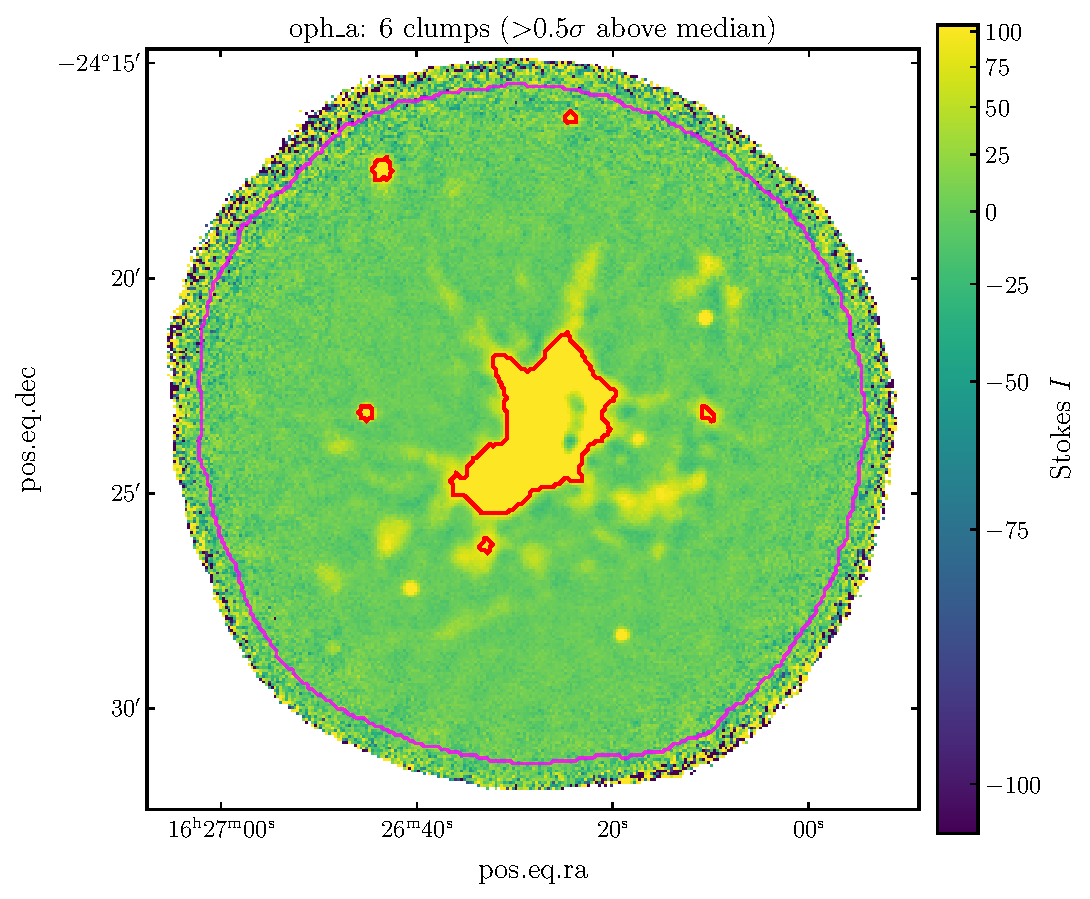
\includegraphics[width=\linewidth]{../plots/oph_a/oph_a_stat_segmentation.pdf} 
    \caption{Segmentation \& Clump Masking} \end{subfigure} \hfill
    \begin{subfigure}{0.48\textwidth} 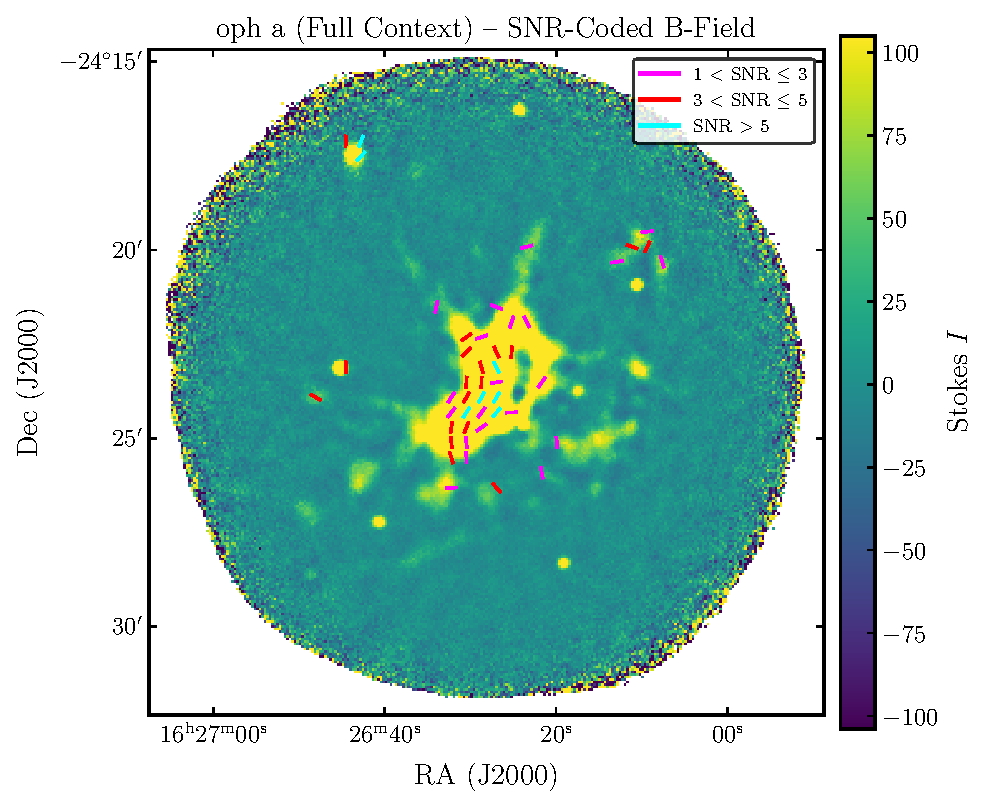
\includegraphics[width=\linewidth]{../plots/oph_a/oph_a_snr_colored_full.pdf} 
    \caption{SNR-Coded B-Field Vectors} \end{subfigure}
    \vspace{0.5cm}
    \begin{subfigure}{0.7\textwidth} 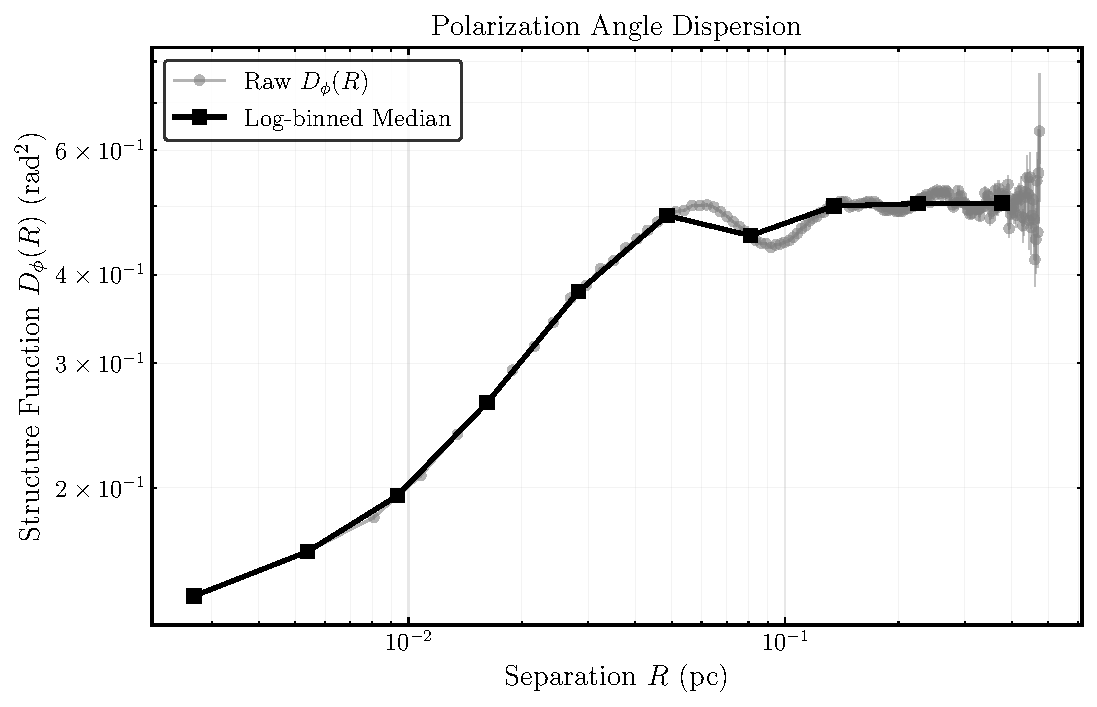
\includegraphics[width=\linewidth]{../plots/oph_a/oph_a_sf.pdf} 
    \caption{Structure Function $D_\phi(R)$} \end{subfigure}
\end{figure}
\newpage
\section*{Target: oph\_b}
\begin{table}[H]
    \centering
    \caption*{Physical Parameters and Noise Methodology}
    \begin{tabular}{lp{10cm}}
        \toprule \textbf{Parameter} & \textbf{Value} \\ \midrule
        Method I & \textbf{Hardware QUALITY Mask} \\
        Method QU & \textbf{Hardware Variance} \\
        Effective Pixels & 1370 \\
        R\_range\_pc & 0.0027 -- 0.4744 \\
        Distance (pc) & 139.00000 \\
        R\_range\_px & [1, 176] \\
        Vector Decimation Step & 3 px \\
        \bottomrule
    \end{tabular}
\end{table}

\begin{figure}[H]
    \centering
    \begin{subfigure}{0.48\textwidth} 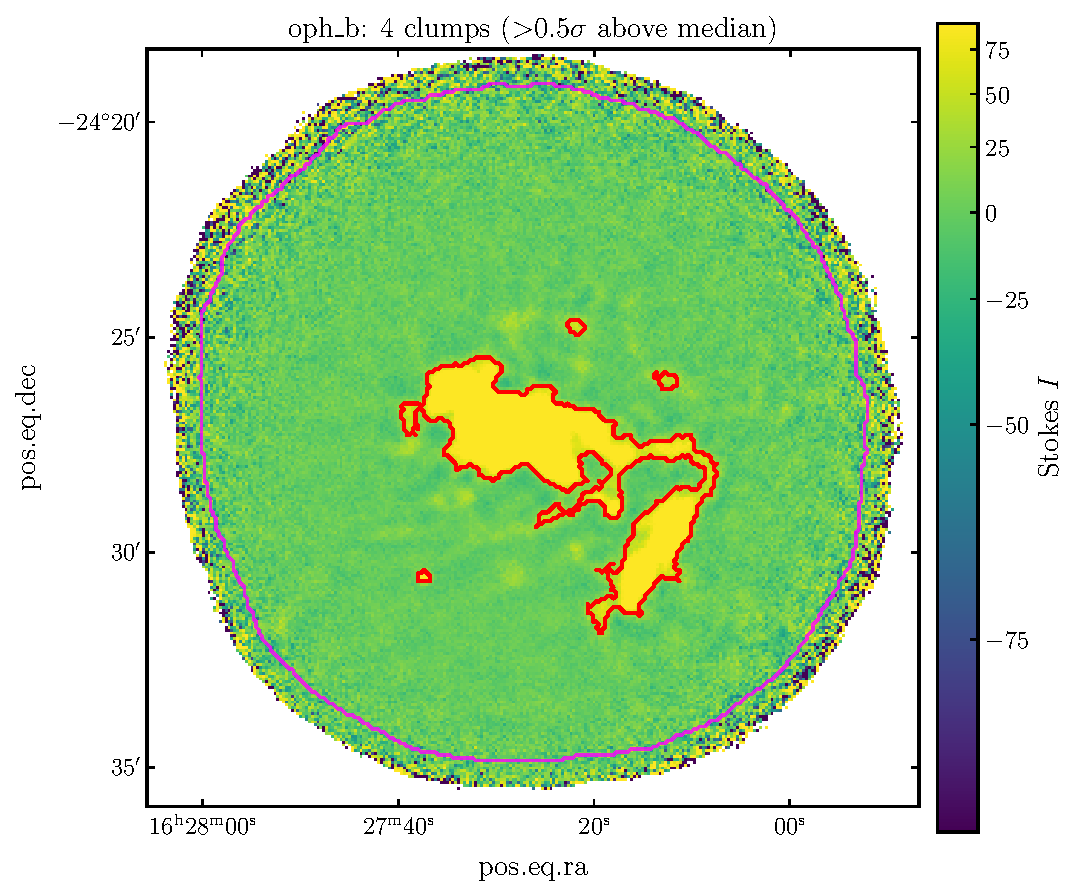
\includegraphics[width=\linewidth]{../plots/oph_b/oph_b_stat_segmentation.pdf} 
    \caption{Segmentation \& Clump Masking} \end{subfigure} \hfill
    \begin{subfigure}{0.48\textwidth} 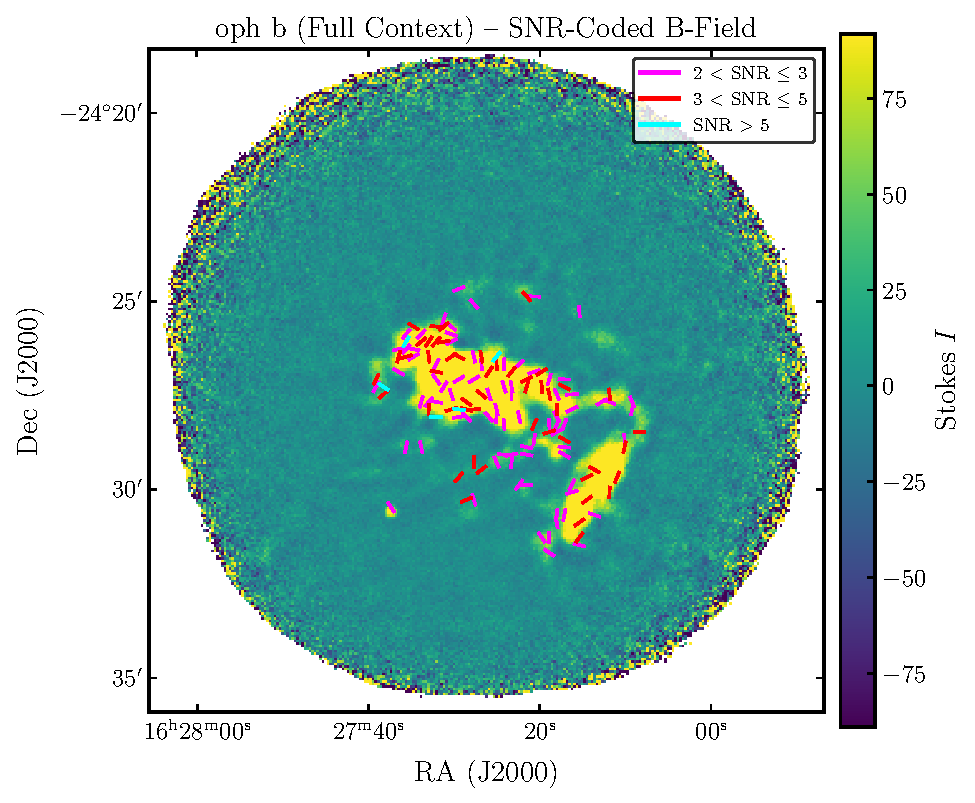
\includegraphics[width=\linewidth]{../plots/oph_b/oph_b_snr_colored_full.pdf} 
    \caption{SNR-Coded B-Field Vectors} \end{subfigure}
    \vspace{0.5cm}
    \begin{subfigure}{0.7\textwidth} 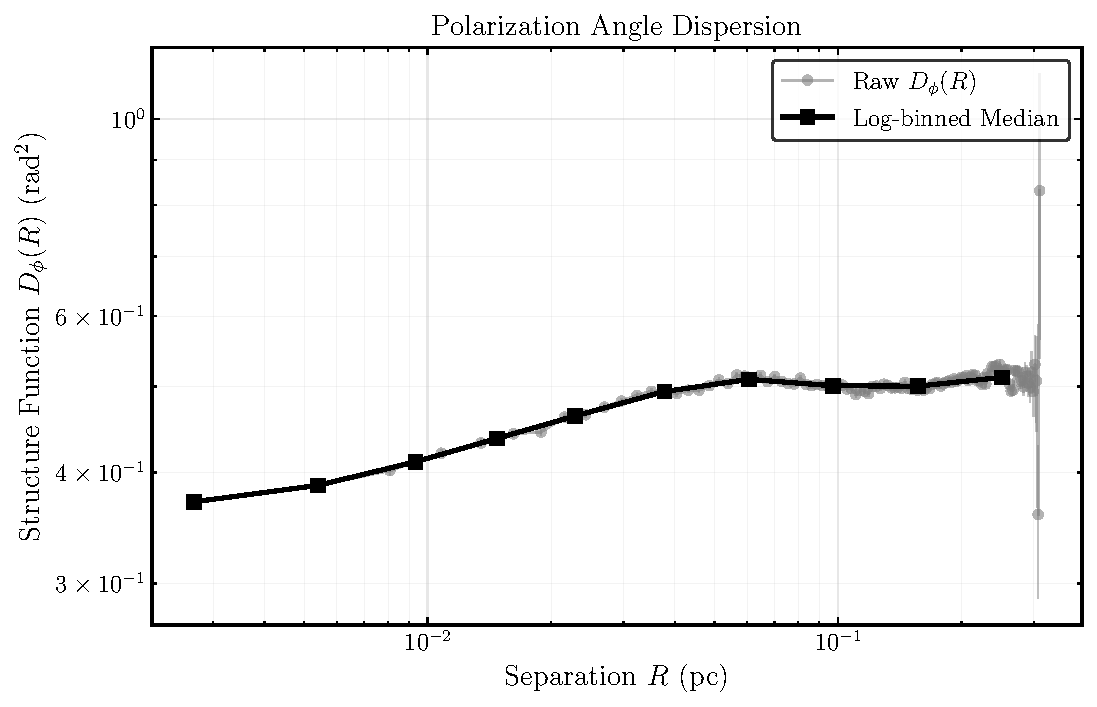
\includegraphics[width=\linewidth]{../plots/oph_b/oph_b_sf.pdf} 
    \caption{Structure Function $D_\phi(R)$} \end{subfigure}
\end{figure}
\newpage
\section*{Target: oph\_c}
\begin{table}[H]
    \centering
    \caption*{Physical Parameters and Noise Methodology}
    \begin{tabular}{lp{10cm}}
        \toprule \textbf{Parameter} & \textbf{Value} \\ \midrule
        Method I & \textbf{Hardware QUALITY Mask} \\
        Method QU & \textbf{Hardware Variance} \\
        Effective Pixels & 921 \\
        R\_range\_pc & 0.0027 -- 0.4744 \\
        Distance (pc) & 139.00000 \\
        R\_range\_px & [1, 176] \\
        Vector Decimation Step & 3 px \\
        \bottomrule
    \end{tabular}
\end{table}

\begin{figure}[H]
    \centering
    \begin{subfigure}{0.48\textwidth} 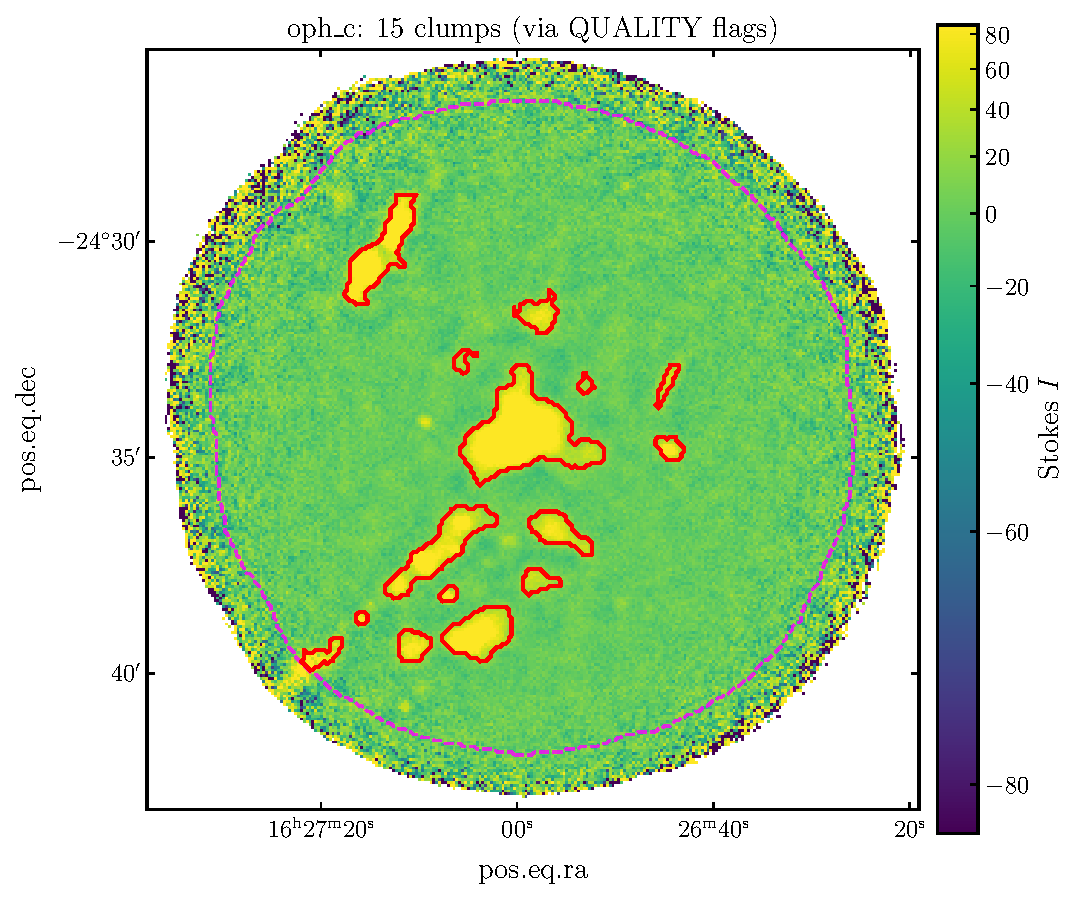
\includegraphics[width=\linewidth]{../plots/oph_c/oph_c_stat_segmentation.pdf} 
    \caption{Segmentation \& Clump Masking} \end{subfigure} \hfill
    \begin{subfigure}{0.48\textwidth} 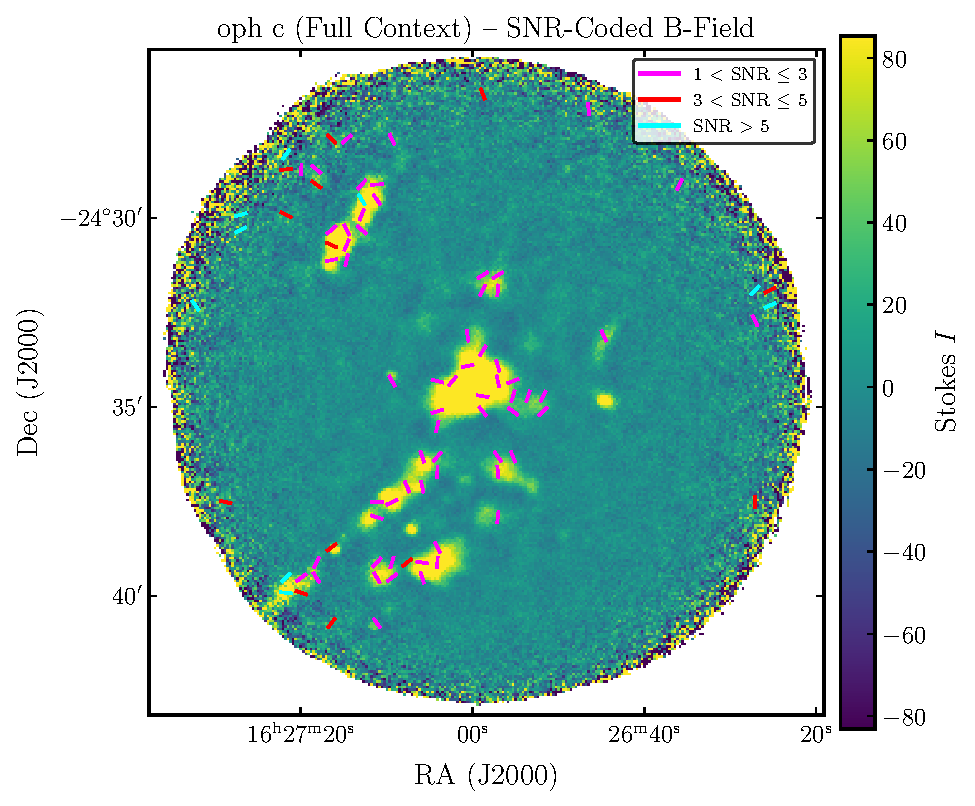
\includegraphics[width=\linewidth]{../plots/oph_c/oph_c_snr_colored_full.pdf} 
    \caption{SNR-Coded B-Field Vectors} \end{subfigure}
    \vspace{0.5cm}
    \begin{subfigure}{0.7\textwidth} 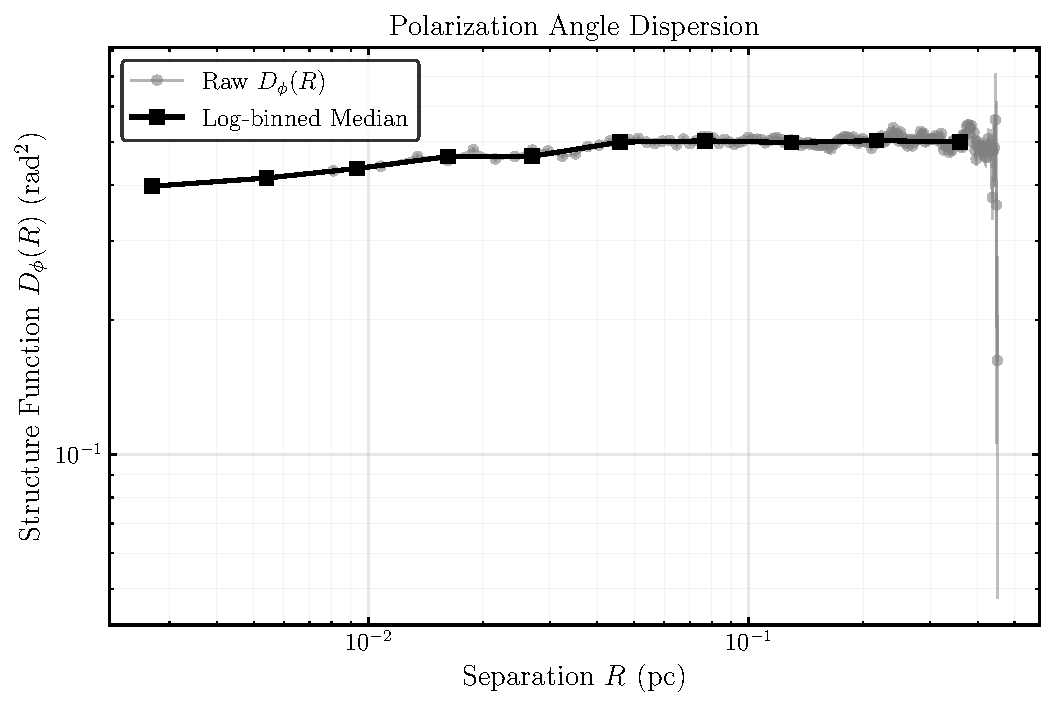
\includegraphics[width=\linewidth]{../plots/oph_c/oph_c_sf.pdf} 
    \caption{Structure Function $D_\phi(R)$} \end{subfigure}
\end{figure}
\newpage
\end{document}